\section{Flyback Converter Design}

\begin{figure}[H]
\begin{center}
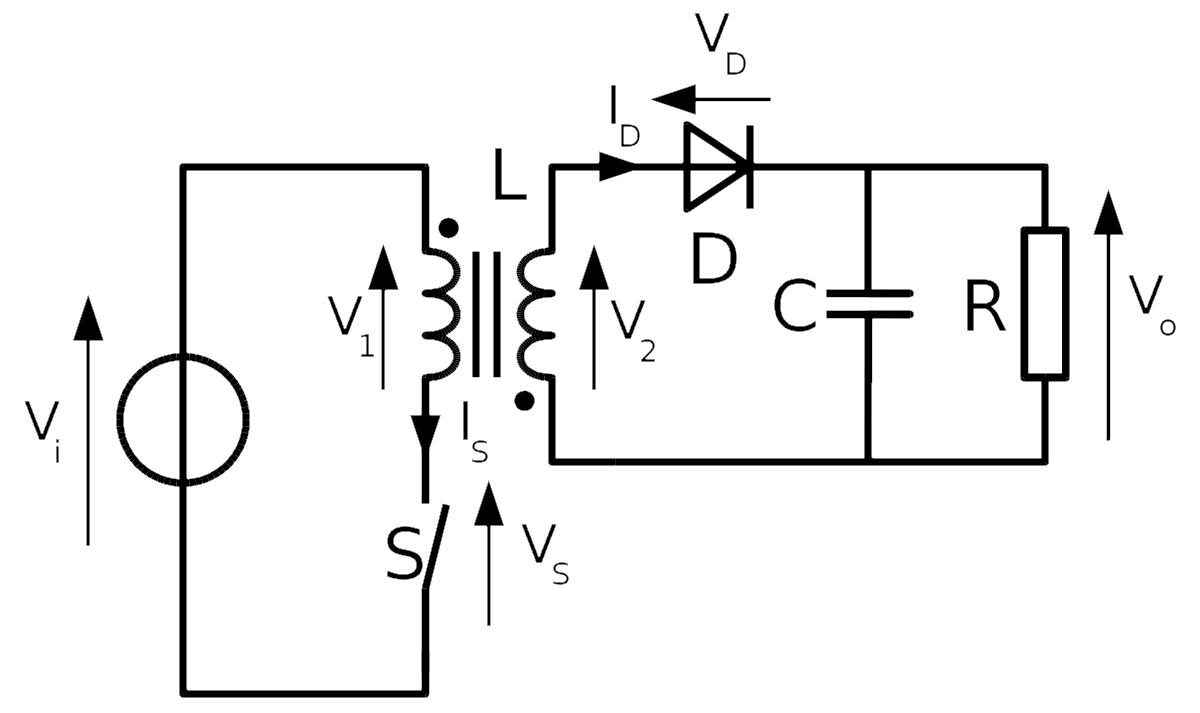
\includegraphics[width=0.6\textwidth]{flybacktop.png}
\caption{Ideal Flyback Converter}
\label{fig:flybacktop}
\end{center}
\end{figure}
An ideal flyback converter topology is given in Figure \ref{fig:flybacktop}. It is a galvanically isolated DC-DC converter with a special feature. That special feature is using the magnetizing inductance of the transformer as an energy storage device, instead of a separate circuit component, which helps reduce the cost, volume and mass of the converter. For our hardware project, we will build a Flyback Converter with extra features to establish the flexibility and performance required to achieve the main requirements and collect bonus points from the Hardware Project. 
\par Our circuit's main controller is UCC28740 by Texas Instruments. It can achieve both current mode and voltage mode control by taking feedback from input and output sides. For UCC28740 to perform properly, the rest of the circuit should be set to achieve DCM operation at all times. UCC28740 can achieve valley switching, which means it will try to switch the MOSFET at the lowest possible voltage than the primary voltage to increase the efficiency. Those voltage levels are called valley points which are bottoms of the voltage swing at the primary, as seen in Figure \ref{fig:valleyswitch}. The lower voltage level is seen because of the ringing when primary current reaches zero. This kind of Flyback Converter called Quasi-Resonant Flyback Converter.

\begin{figure}[H]
\begin{center}
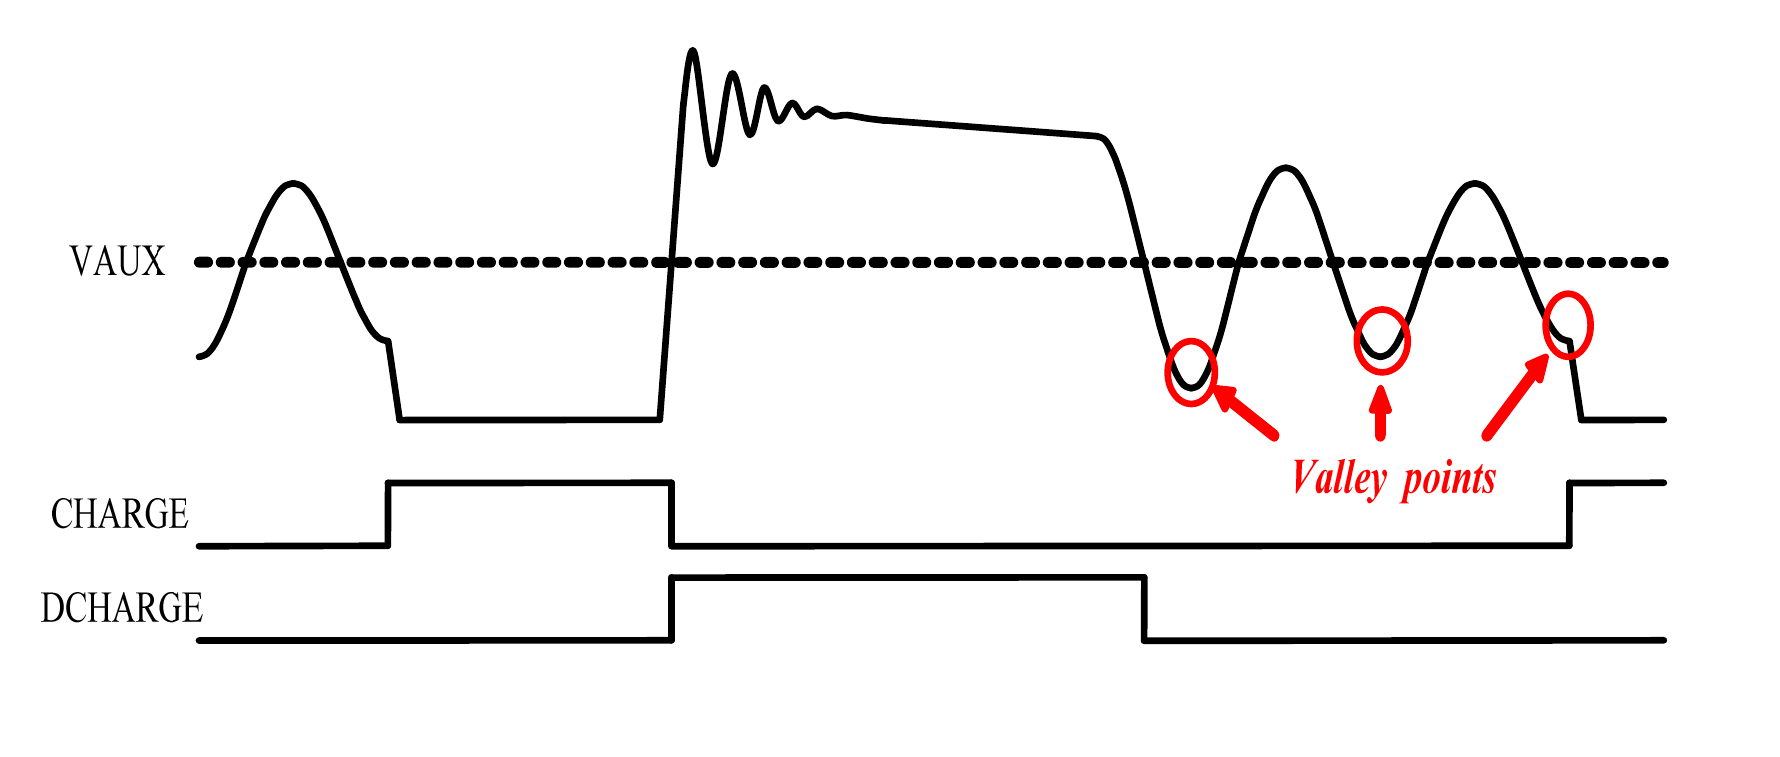
\includegraphics[width=0.6\textwidth]{valleyswitch.png}
\caption{Vallet Points of a Quasi-Resonant Flyback Converter}
\label{fig:valleyswitch}
\end{center}
\end{figure}

To be able to handle synchronous switching, UCC24636 by Texas Instruments will be used at the secondary side. The reference design for the mentioned ICs is given in Figure \ref{fig:refdesign}.

\begin{figure}[H]
\begin{center}
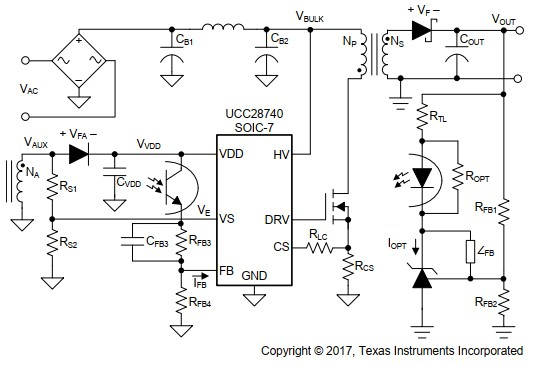
\includegraphics[width=0.6\textwidth]{refdesign.jpg}
\caption{Reference Flyback Converter Design with UCC28740}
\label{fig:refdesign}
\end{center}
\end{figure}


\subsection{Design Goals}
Complying with the specifications given in the project description, Table \ref{tab:specs} is prepared as a summary. Our design must accomplish the given performance measures. In addition to these, the circuit must employ a closed-loop control. Furthermore, to maximize the functionality and gain bonus points we aimed to go for each positive bonus parts described.
\begin{table}[H]
\centering
\caption{Project Specifications}
\begin{tabular}{|c|c|c|c|c|c|}
\hline
\multicolumn{2}{|c|}{\textbf{Paremeter}}   & \textbf{Min}          & \textbf{Typical}      & \textbf{Max}          & \textbf{Unit}         \\ \hline
\multicolumn{2}{|l|}{\textbf{INPUT}}       & \multicolumn{1}{l|}{} & \multicolumn{1}{l|}{} & \multicolumn{1}{l|}{} & \multicolumn{1}{l|}{} \\ \hline
$V_{in}$  & Input Voltage                       & 24                    & 36                    & 48                    & VDC                   \\ \hline
\multicolumn{2}{|l|}{\textbf{OUTPUT}}      &                       &                       &                       &                       \\ \hline
$V_{out}$ & Output Voltage                      & 14.4                  & 15                    & 15.6                  & VDC                   \\ \hline
$I_{out}$ & Output Current                      & -                     & 3.75                  & -                     & A                     \\ \hline
$P_{out}$ & Output Power                        &                       & 60                    &                       & W                     \\ \hline
     & Line Regulation                     &                       &                       & 2                     & \%                    \\ \hline
     & Load Regulation                     &                       &                       & 2                     & \% 
     \hline
\label{tab:specs}
\end{tabular}
\end{table}
\subsection{Parameter Calculations}
\subsubsection*{Duty Cycle, Turns Ratio, Primary Inductance, Peak Primary Current}
Since the target maximum switching frequency imposed by the limitations of our controllers, it is designated as 45 kHz. $D_{MAGCC}$ is defined as `The secondary diode conduction duty-cycle limit in CC mode, 0.425. which is a device parameter to make sure the transformer is demagnetized and DCM is established. Assuming 500 kHz as the DCM resonance frequency, the times it takes to reach the first valley of $V_{DS}$, $t_R$ should be substracted so that valley switching can be made possible too. To find the maximum duty cycle for constant CCM operation,
\begin{align*}
D_{MAX}&=1-D_{MAGCC}-f_{MAX}\times\frac{t_R}{2}\\
D_{MAX}&=1-0.425-45kHz\times \frac{2 \mu s}{2}=0.53
\end{align*}
\par Since $D_{MAX}$ is known, maximum primary to secondary turns ratio can be determined with the following equation:
\begin{align*}
    N_{PS,MAX}=\frac{D_{MAX} V_{DC,min}}{D_{MAGCC}(V_{O}+v_F})=\frac{0.53\times 24}{0.425*(15.7)}=1.906
\end{align*}

Since the voltage at the current sense feedback pin of the controller, $V_CST$ is limited, first we need to determine de $R_{CS}$ to limit the the primary peak current,$I_{PP}$.
\begin{align*}
    R_{CS}&=\frac{V_{CCR}N_{PS}}{2I_{O}}\sqrt{\eta_{transformer}}=74.3m\Omega\\
    I_{PP,MAX}&=\frac{V_{CST,MAX}}{R_{CS}}=\frac{0.773}{0.0746}=10.4A
\end{align*}
Where $V_{CCR}$ is a device parameter called constant-current regulation factor and is equal to 330mV.
To compansate the voltage ripples on the input capactiors, a factor of 0.6 is used. 

%\begin{align*}
%    I_{PPK}=\frac{2P_{out}}{\eta V_{in,min}\sqrt{2}\times 0.8D_{MAX}}=\frac{2\times 60W}{0.85\times %24\sqrt{2}\times 0.6\times 0.53}=13.08A
%\end{align*}


\par To ensure enough energy can be stored in the transformer and DCM operation is established, primary inductance should be specified properly It should be noted that the transformer will cause losses so they need to taken into consideration too. Assuming \% efficiency, magnetizing inductance is calculated.
\begin{align*}
    L_P=\frac{2(V_O+V_F)I_O}{\eta _{transformer}I_{PP,MAX}^2f_{MAX}}=\frac{2\times 15.7\times 4}{0.9\times 10.4^2\times f_{MAX}}=28.67\mu H
\end{align*}
Lastly, since we will need an auxiliary winding to power the controller to sense the primary voltage and utilize low voltage lockout, turns ratio of it should be calculated too. Assuming the lockout voltage to be 15V, and auxiliary diode voltage drop to be 0.5 Volts. Lastly, the upper limit for auxiliary to secondary turns ratio is calculated according to the lowest supply voltage of the controller, $V_{DD,off}$
\begin{align*}
N_{AS,MAX}&=\frac{V_{DD,min}+V_{FA}}{V_O+V_F}=\frac{7.75+0.5}{15+0.7}=0.525\\
N_{PA,MAX}&=\frac{1.9}{0.525}=3.62
\end{align*}

\subsection{Transformer Parameter Verification}
To be able to choose our components properly, the stresses on them should be calculated to make an informed decision. Turns ratio of the transformer affects the peak voltages on the rectifiers. Also, demagnetization and MOSFET on times are should be verified so that the values are in the internal timing limits of our controller.
Reverse voltages on primary and secondary rectifiers are,
\begin{align*}
V_{Reverse,secondary}&=\frac{V_{IN,MAX\sqrt{2}}}{N_{PS}}+V_{O,MAX}=77.8V\\
V_{Reverse,primary}&=\frac{V_{IN,MAX}}{N_{PA}}+V_{VDD}=23.25V
\end{align*}
For MOSFET $V_{DS}$ peak voltage calculation;
\begin{align*}
    V_{DS,peak}=V_{IN,MAX}+(V_O+V_F)N_{PS}=97V
\end{align*}
To find our circuits ON time and Demagnetization times,
\begin{align*}
t_{ON,min}=\frac{L_P}{V_{IN,MAX}}\frac{I_{primary,MAX}}{4}=1.51\mu s\\
t_{Dmag.Min}=\frac{t_{ON,min}V_{IN,MAX}}{N_{PS}(V_O+V_F)}=2.9\mu s
\end{align*}
The minimum required ON time for our controllers is indicated as 280 nS and minimum Demagnetizing time is specified as 2.4 $\mu$S. Both criteria are satisfied and our circuit can operate in nominal conditions.
\subsection{Magnetic Design}
Firstly, the shape of the transformer core is selected as an E-core. Since E-cores can be winded better than toroid cores. To have enough turn numbers on both primary and secondary side, KOOL MU 2510 E CORE(00K2510E090) is selected. Cross-section area of the core is important for turn numbers and core area of the KOOL MU 2510 E CORE is small enough to have 10 turns on the primary side. Parameters of the chosen E-core is given below;
\begin{align}
    A_e &= 35mm^2(Cross Section Area)\\ l_e &= 48.5 mm (Path Length) \\\mu_c &= 90 (Relative Permeability) \\ B_c &= 1 T (Saturation Flux Density) \\ Weight &= 5.9 g and V_e=1870 mm^3 (Volume) 
\end{align}
According to chosen core secondary turn numbers was calculated.
\begin{align}
    N_S&=\frac{L_P\times I_{peak}}{n\times B_m \times A_e}\\
    N_S&=\frac{28.67\times 10^{-6} \times 10.8 }{1.9 \times 1 \times 35 \times 10^{-6}}=5.2 turns
\end{align}
Ratio of the primary turn numbers to secondary turn numbers is calculated, so primary turn number is given below;
\begin{align}
    N_P= n\times N_S = 1.9 \times 5.2 = 10 turns
\end{align}
In this flyback converter design, UCC28740 analog controller is chosen to control the output voltage and current. To supply V$CC$(7.75V) to UCC28740 analog controller, there is required auxiliary winding come from the transformer. The turn number of the auxiliary winding is calculated below;
\begin{align}
    N_{VCC}= \frac{V_{CC}}{V_O+V_F}\times N_S = \frac{7.75}{12+0.7}\times N_S= 3 turns
\end{align}
There is a core gap on the E-core. Core gap is crucial because magnetic flux intensity can be controlled by the core gap. If there is smaller gap than required, the core can be saturated and transformer could not work properly. Also the other components of the flyback converter can be damaged due to overload. Required core gap is calculated to have optimum magnetic design. Calculation of the core gap is given below;
\begin{align}
    gap=\frac{\mu_0\times N_P{^2}\times A_e }{L_P}-\frac{I_e}{\mu_c}=\frac{1.256\times 10^{-6}\times 10{^2}\times 35\times 10^{-6}}{28.67\times 10^{-6}}-\frac{48.5\times 10^{-3}}{90}=1.35\times 10^{-3}m
\end{align}
To check the calculated values given equations is done. Magnetic flux intensity is crucial, since if it is higher than the saturation level of the core, saturation level of the chosen core is 1 Tesla.
\begin{align}
    B=\frac{\mu_0\times N_P\times I_P}{\frac{I_e}{\mu_c}+gap}&=\frac{1.256\times 10^{-6}\times 10\times 10.8}{\frac{48.5\times 10^{-3}}{90}+3.85\times 10^{-3}}=0.95\\
    V_r&=\frac{N_P}{N_S}\times (V_O+V_F)=24.13 V
\end{align}
0.95 Tesla is lower than saturation level of the core so it is acceptable. Also duty ratio must be lower than 0.53. To check duty ratio of the design, D is calculated below;
\begin{align}
    D=\frac{V_r}{V_r+V{_dc(min)}}=0.5
\end{align}

